\documentclass[aspectratio=169]{beamer}
\usetheme{Madrid}
\usecolortheme{default}
\setbeamertemplate{navigation symbols}{}
\setbeamertemplate{caption}[numbered]

\title{Realtime ASR Project Background}
\author{CS5296 Group 7}
\date{\today}

\begin{document}

\begin{frame}{Project Background and Problem Context}
\small{\textbf{Realtime ASR Project Background} \hfill CS5296 Group 7}

\vspace{0.6em}
\textbf{Goal:} Build a practical, realtime speech-to-text web system that supports downstream understanding.

\vspace{0.4em}
\textbf{Why this project matters}
\begin{itemize}
  \item Traditional transcription workflows are often offline and slow.
  \item Real deployments need low latency, stability, and easy operations.
  \item Teams also need immediate value after transcription, such as summary and rewriting.
\end{itemize}

\vspace{0.4em}
\textbf{Project objectives}
\begin{itemize}
  \item Stream browser microphone audio to backend in realtime.
  \item Produce live transcripts using Vosk ASR.
  \item Provide one-click post-processing: summarize and rewrite.
  \item Support cloud deployment with observability.
\end{itemize}
\end{frame}

\begin{frame}{System Background and Architecture Rationale}

\begin{figure}
  \centering
  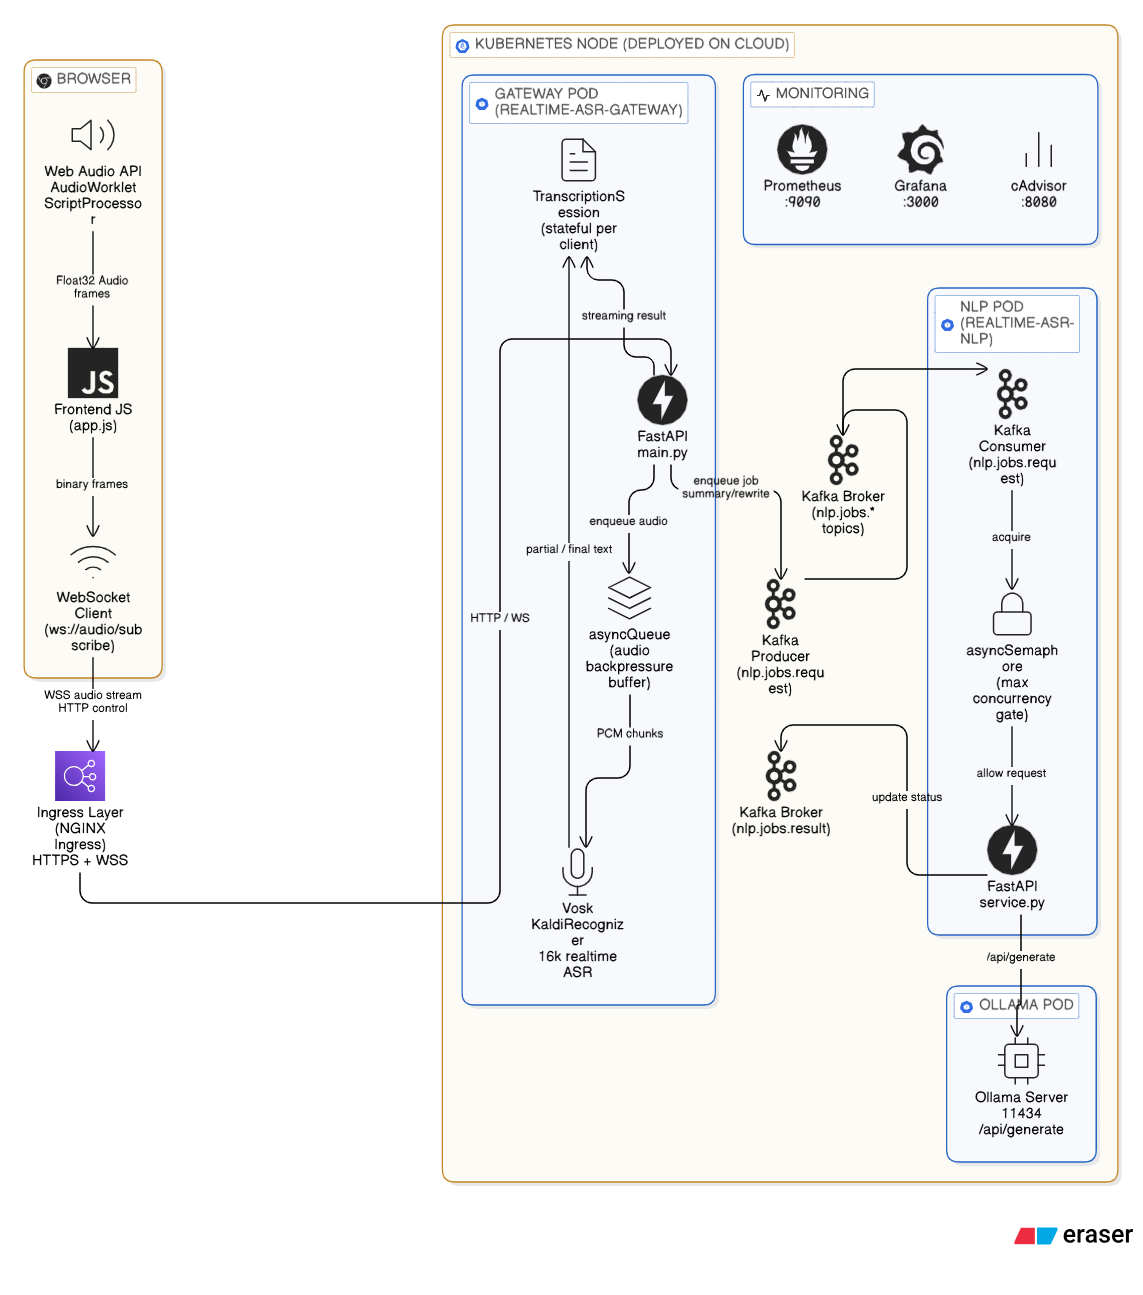
\includegraphics[width=0.35\linewidth]{figures/image1.png}
  \caption{End-to-end architecture of Live ASR stream processing pipeline}
  \label{fig:system-architecture}
\end{figure}
\end{frame}

\begin{frame}{Summary of Tuning Results and Final Configuration}
    \textbf{Deployment targets}
\begin{itemize}
  \item Docker Compose for fast local iteration.
  \item Kubernetes (k3s) for cloud deployment on Alibaba ECS.
\end{itemize}

\vspace{0.4em}
\textbf{Operational concerns observed in practice}
\begin{itemize}
  \item HTTPS and ingress configuration for secure microphone access.
  \item Resource pressure from larger ASR models under limited ECS CPU and memory.
  \item WebSocket session stability under real network and load conditions.
\end{itemize}

\vspace{0.4em}
\textbf{Supporting platform capabilities}
\begin{itemize}
  \item Prometheus and Grafana for monitoring and performance visibility.
  \item Configurable runtime knobs (queue size, concurrency, model path).
  \item Scripted deployment to improve reproducibility and onboarding.
\end{itemize}
\end{frame}

\begin{frame}{ASR Result}
\textbf{ASR accuracy overview}

\begin{figure}
  \centering
  
\includegraphics[width=0.62\linewidth]{\detokenize{figures/asr word error rate.png}}
  \caption{ASR Word Error Rate (WER) comparison under evaluated settings}
  \label{fig:asr-wer-results}
\end{figure}

\small{The measured WER trend indicates the selected setup provides the best accuracy-stability balance for this deployment profile.}
\end{frame}

\begin{frame}{Deployment Background and Engineering Constraints}
\vspace{0.4em}
\textbf{Practical implication}
\begin{itemize}
    \item Simulate 2-node deployment with KIND (Kubernetes in Docker) and load testing script.
  \item Which configuration gave the best balance of responsiveness and stability under constrained resources?
\end{itemize}

% \vspace{0.3em}
% \small{Primary benchmark view is shown in Figure~\ref{fig:perf-main}.}

% \begin{itemize}
%   \item Simulate 2-node deployment with KIND (Kubernetes in Docker) and load testing script.
% \end{itemize}

\begin{figure}
  \centering
  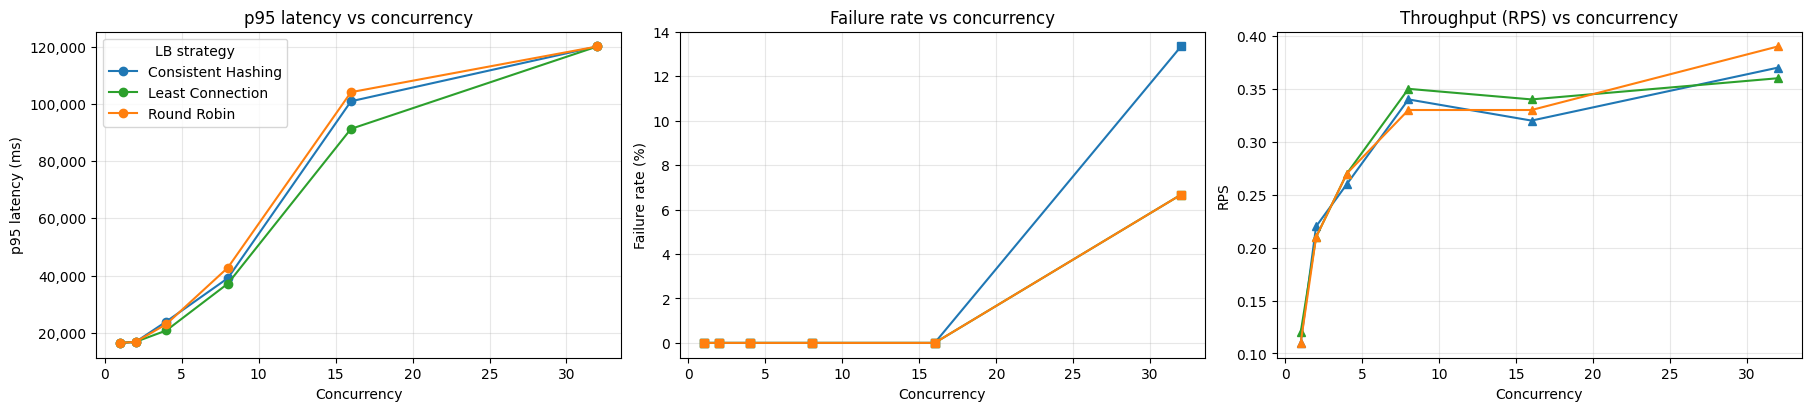
\includegraphics[width=0.72\linewidth]{figures/image2.png}
  \caption{Benchmark comparison of single-server double-node tuning candidates}
  \label{fig:perf-main}
\end{figure}
\end{frame}

\begin{frame}{Performance Tuning Results for Single-Server Deployment (Cont.)}
\small{Additional profiling evidence is shown in Figure~\ref{fig:perf-queue} and Figure~\ref{fig:perf-semaphore}.}

\begin{columns}[T,onlytextwidth]
\column{0.49\textwidth}
\begin{figure}
  \centering
  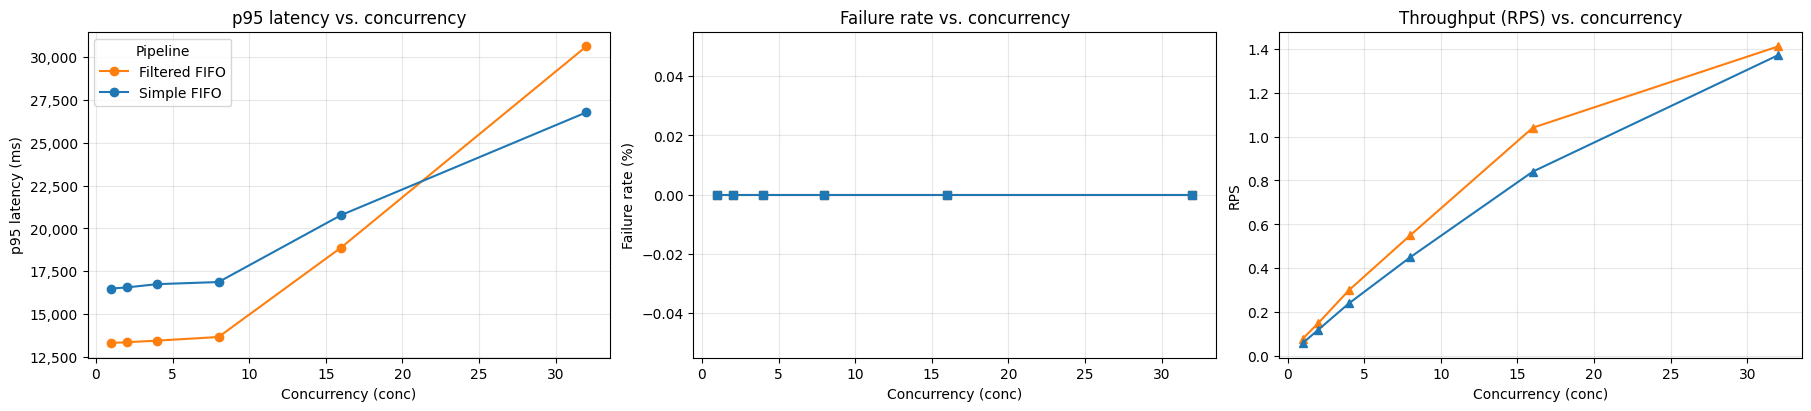
\includegraphics[width=\linewidth]{figures/image3.png}
  \caption{Chunk queue method comparison under sustained traffic}
  \label{fig:perf-queue}
\end{figure}

\column{0.49\textwidth}
\begin{figure}
  \centering
  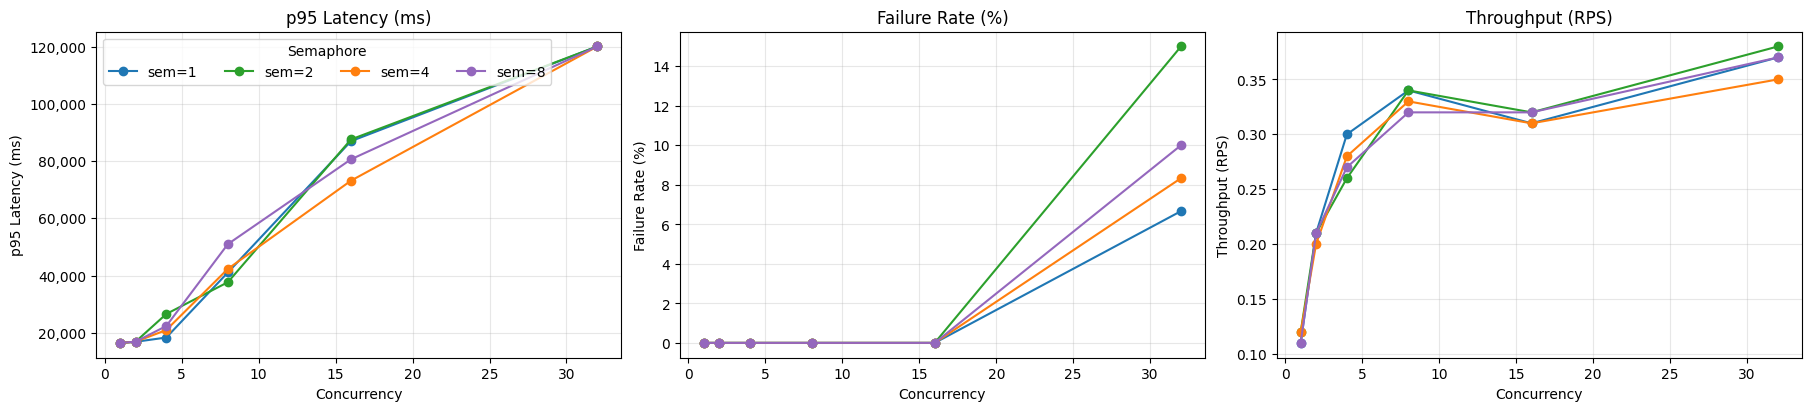
\includegraphics[width=\linewidth]{figures/image4.png}
  \caption{Semaphore sweep: throughput vs. stability trade-off}
  \label{fig:perf-semaphore}
\end{figure}
\end{columns}
\end{frame}

\begin{frame}{Performance Tuning Results for Single-Server Deployment}
\textbf{What we tested}
\begin{itemize}
  \item Load balancing algorithms across gateway replicas.
  \item Different audio chunk queue handling methods.
  \item Concurrency control with semaphore limits.
\end{itemize}

\vspace{0.4em}
\textbf{Key finding}
\begin{itemize}
  \item For stateless single-server single-node deployment, the most stable setup is:
  \item Semaphore = 1
  \item Load balancing algorithm = least connection
\end{itemize}
\end{frame}

\end{document}
